\subsubsection{Thiết kế hệ thống}
Nhằm đảm bảo hệ thống có khả năng bảo trì, mở rộng và kiểm thử dễ dàng, kiến trúc của dự án được thiết kế theo mô hình \textbf{Layered Architecture}. Đây là một mô hình kiến trúc phổ biến và vững chắc, giúp tách bạch rõ ràng các mối quan tâm của ứng dụng thành các lớp logic riêng biệt. Luồng xử lý chính của hệ thống tuân theo quy tắc phụ thuộc chặt chẽ: một lớp ở trên chỉ có thể giao tiếp với lớp ngay bên dưới nó. Dữ liệu yêu cầu sẽ đi từ lớp trên cùng xuống các lớp dưới để xử lý và truy xuất dữ liệu, sau đó dữ liệu phản hồi sẽ được trả ngược lên trên.
\begin{figure}[H]
    \centering
    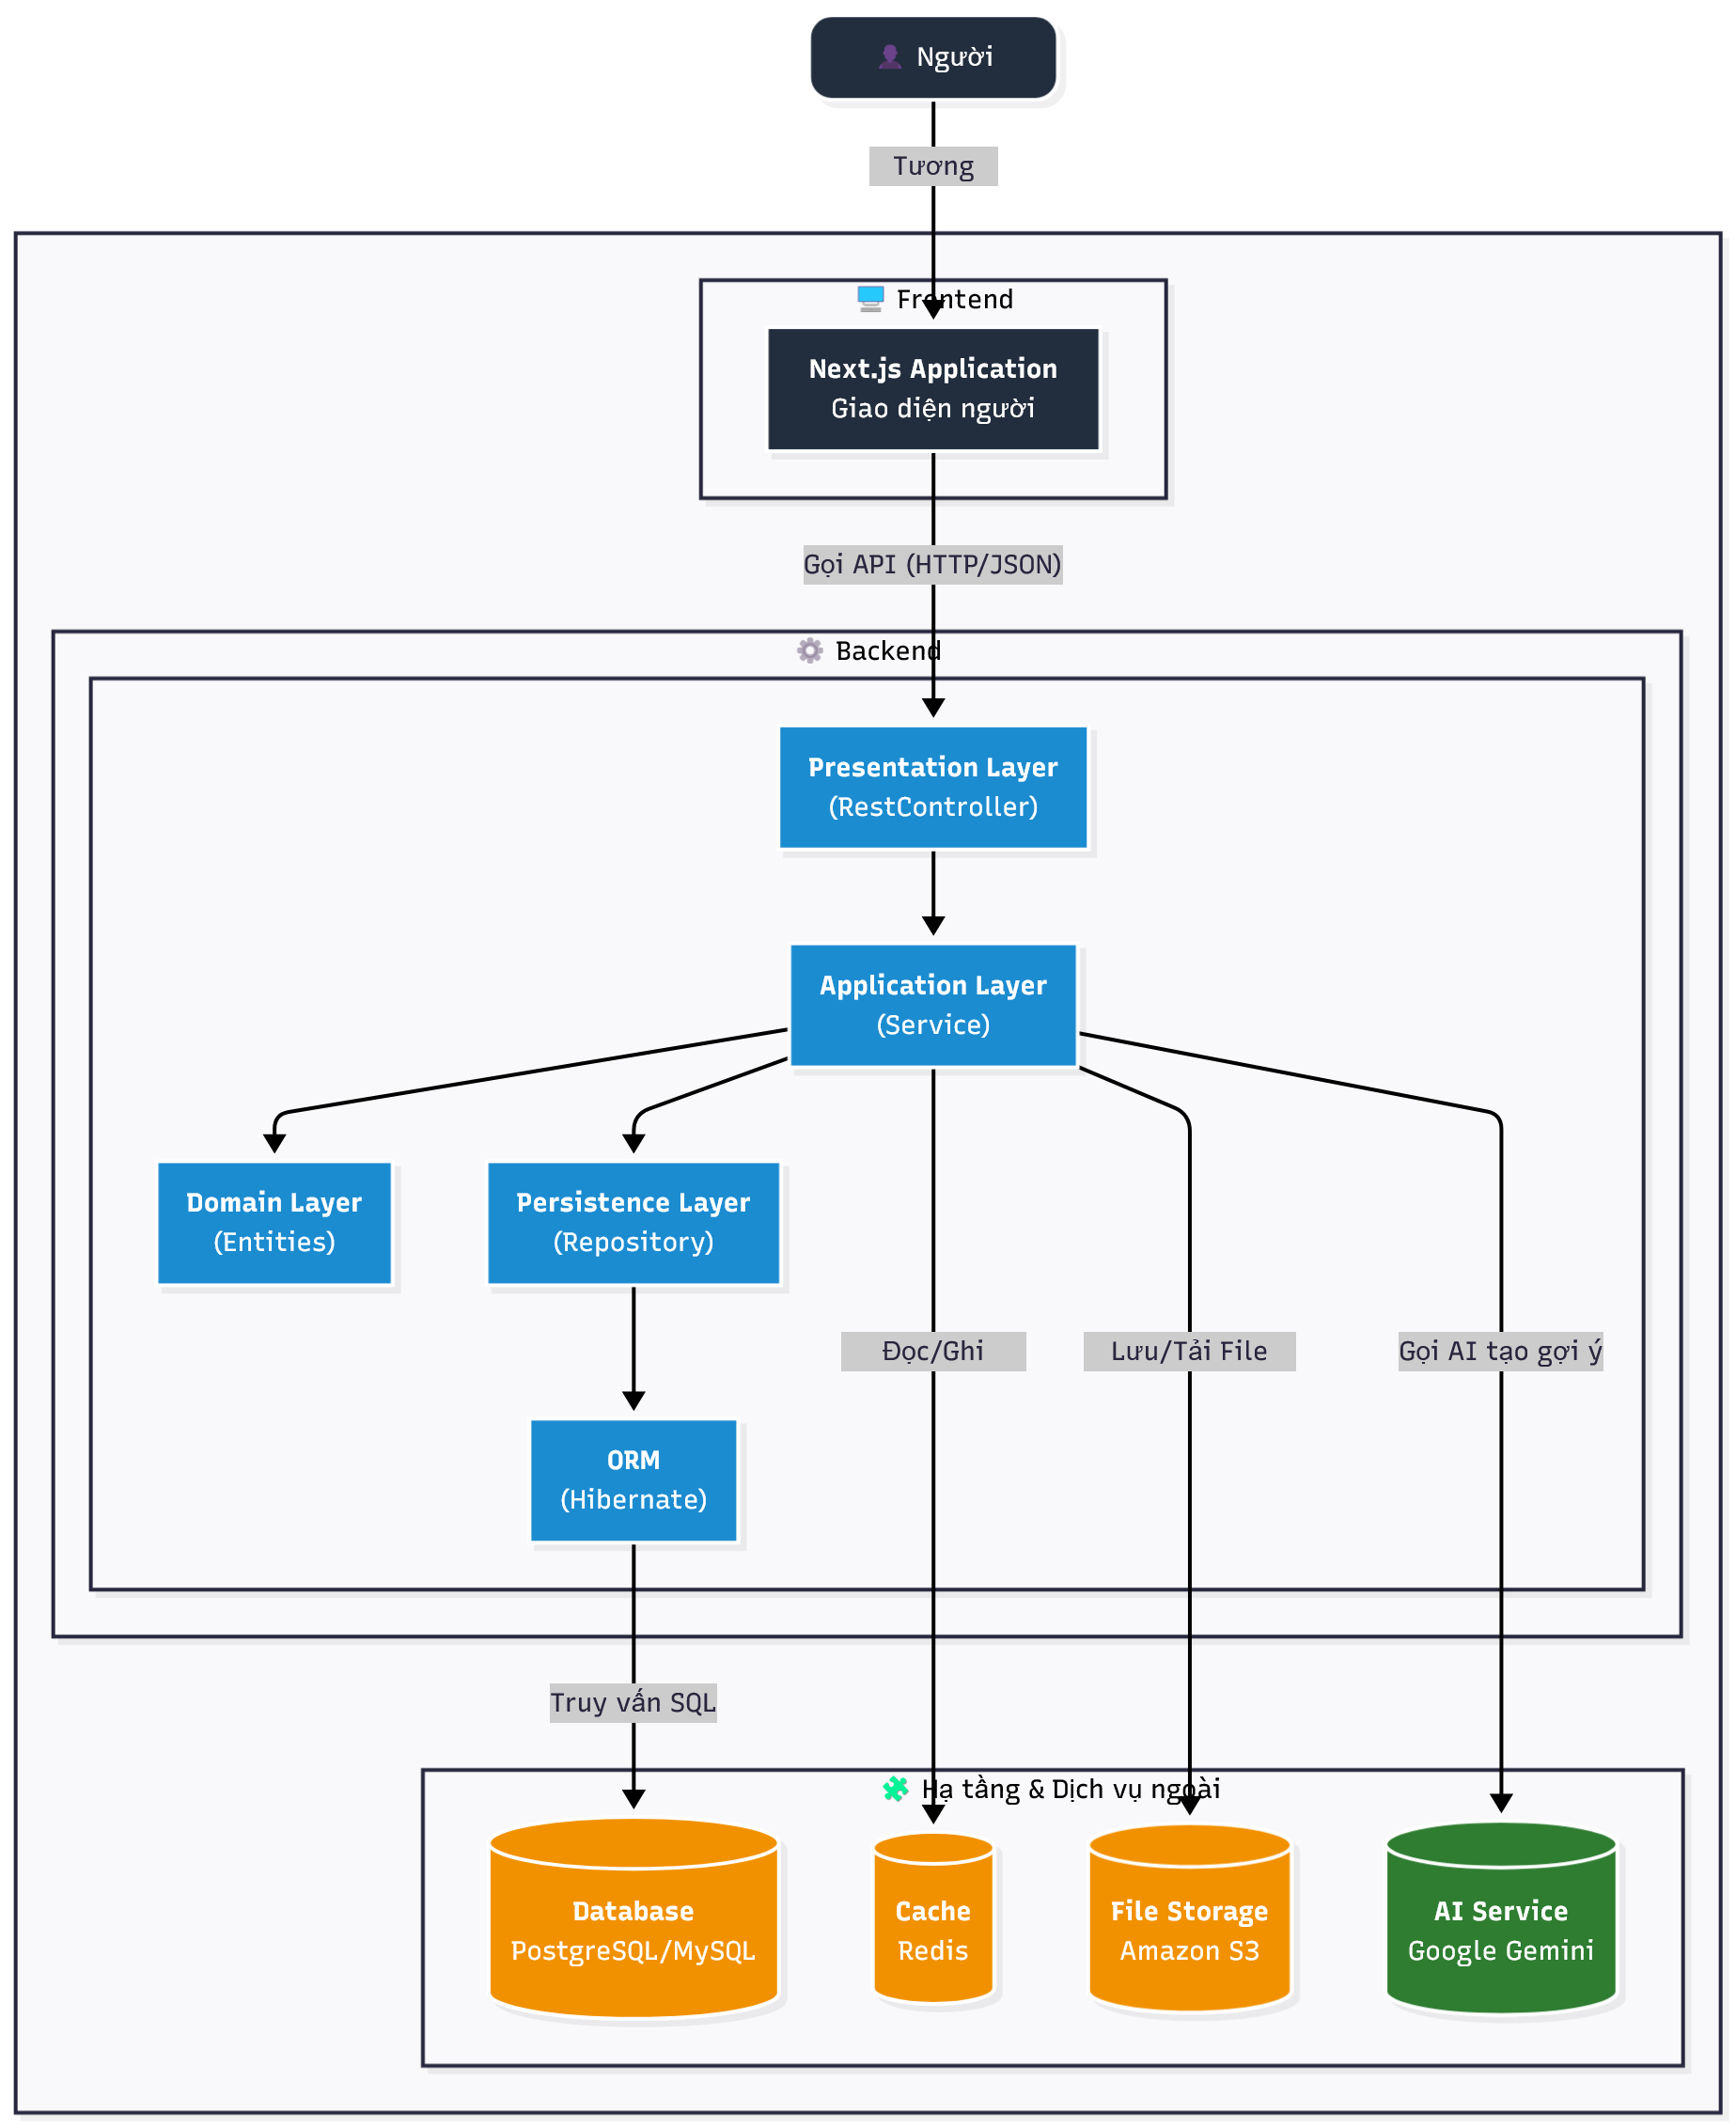
\includegraphics[width=0.9\textwidth]{Images/7. System Design/Kiến trúc hệ thống.png}
    \caption{Kiến trúc hệ thống}
    \label{fig:overview_system}
\end{figure}
Các tầng trong kiến trúc hệ thống:
\begin{itemize}
    \item \textbf{User Interface:} hiển thị giao diện và tiếp nhận tương tác trực tiếp từ người dùng.
    \item \textbf{Presentation Layer:} tiếp nhận, xác thực và điều hướng các yêu cầu (HTTP/WebSocket) từ client.
    \item \textbf{Application Layer:} thực thi logic nghiệp vụ chính và điều phối các tác vụ của hệ thống.
    \item \textbf{Domain Layer:} định nghĩa các thực thể, quy tắc và mô hình kinh doanh cốt lõi.
    \item \textbf{Persistence Layer :} trừu tượng hóa các hoạt động truy xuất dữ liệu thông qua các interfaces.
    \item \textbf{Infrastructure Layer:} cung cấp các chức năng kỹ thuật và giao tiếp với các hệ thống bên ngoài (AI, Cache, Email...).
    \item \textbf{Data Layer:} Lưu trữ vật lý toàn bộ dữ liệu của ứng dụng.
\end{itemize}


